\chapter{Improving Build Times}
The project groups want the build times on Jenkins to be faster. When multiple changes are pushed to the master branch within a short space of time, they will create congestion the build queue. This means that even though the build itself may take only a few minutes, the time it takes from push to finished build may be much longer.

To identify in which parts of the build process to make faster, we measure the time different parts of the Launcher project take. The Launcher project is the main application which depends on many other subprojects. The timings are measured on the Jenkins server and shown in \figureref{fig:launcher_build_times_1}. The shows the build timings of the Launcher application and the different subprojects (\emph{Oasis-lib, Giraf-Component, Local-db, Barcode-scanner, and Metadata}), as well as the startup time for the emulator. As can be seen, the emulator and the Giraf-component and Oasis-lib projects have the most significant influence on build times. These three parts use about \SI{90}{\percent} of the total build time.

To understand which parts of the subprojects that take time, we measure the individual build steps (tasks) performed during a build. These can be seen in \appendixref{app:build_times}. The reason that the Oasis-lib subproject takes a long time to build is that it contains a great number of tests which run on the emulator. These tests are run every time a project depending on Oasis-lib builds --- even though the library itself has not been updated. The most significant task when building the Giraf-Component library is the test task as well. However, the Giraf-Component library only contains one simple test, so we do not expect the actual test execution time to use much of this time. Instead, we expect it to be caused by the order in which projects are tested. When preparing the tests, the tests from all projects are combined into a single Android application package (APK-file). The first test task run is responsible for installing this application on the emulator, while the subsequent test tasks can skip this step. Because the Giraf-components project is the first in the sequence of libraries to be tested, this task also installs the tests on the emulator which is likely to take some time.
\todo{Overvej flere målinger og tag gennemsnit}
\begin{figure}
  \centering
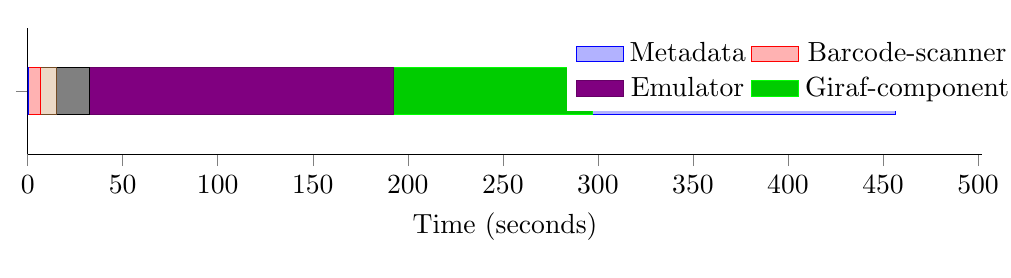
\begin{tikzpicture}[trim axis left, trim axis right]
  \begin{axis}[
    xbar stacked,
    scale only axis,
    width=\textwidth,
    axis y line*= none, axis x line*= bottom,
    %xmajorgrids = true,
    ytick = data,
    yticklabels = {},
    tick align = outside,
    %xtick pos = left,
    bar width=6mm,
    y=8mm,
    %nodes near coords,
    legend style={
      legend columns=4,
      anchor=north,
      yshift=0ex,
      xshift=0ex,
      draw=none
      %legend cell align=left
    },
    area legend,
    xlabel = {Time (seconds)},
    xmin = 0
  ]
    \addplot coordinates
    {(0.2,0)};
    \addlegendentry{Metadata}
    \addplot coordinates
    {(6.625,0)};
    \addlegendentry{Barcode-scanner}
    \addplot coordinates
    {(8.393,0)};
    \addlegendentry{Launcher}
    \addplot coordinates
    {(17.223,0)};
    \addlegendentry{Local-db}
    \addplot coordinates
    {(160.000,0)};
    \addlegendentry{Emulator}
    \addplot coordinates
    {(104.696,0)};
    \addlegendentry{Giraf-component}
    \addplot coordinates
    {(159.497,0)};
    \addlegendentry{Oasis-lib}
    %\legend{Test, test, test, test, test, test}
  \end{axis}
\end{tikzpicture}
\caption{Timings during build of the Launcher project before updating emulator plugin.}\label{fig:launcher_build_times_1}
\end{figure}

To improve the overall build times, we look at how to speed up the emulator and to avoid running tests on the dependencies every time a project is build. We first update the Android Emulator Jenkins plugin to a new version with improved emulator stability. We do this to ensure that we do not work on improving parts which are already improved in the most recent version of the plugin. After updating, we measure the build times again. As shown in \figureref{fig:launcher_build_times_2}, the emulator startup time is significantly increased. Because of this, the emulator startup time is no longer a concern, and we focus solely on decreasing the subproject build times.
\begin{figure}
\centering
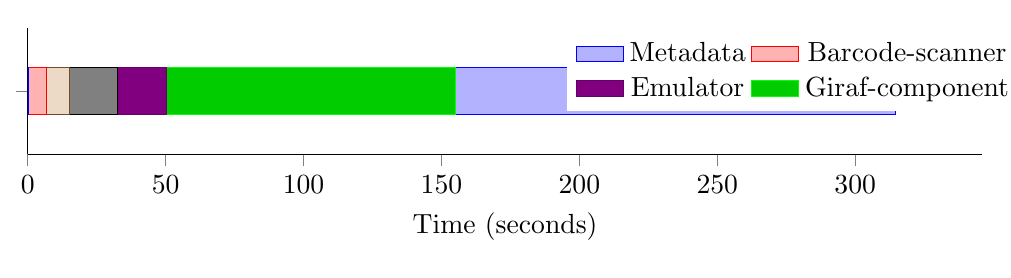
\begin{tikzpicture}[trim axis left, trim axis right]
  \begin{axis}[
    xbar stacked,
    scale only axis,
    width=\textwidth,
    axis y line*= none, axis x line*= bottom,
    %xmajorgrids = true,
    ytick = data,
    yticklabels = {},
    tick align = outside,
    %xtick pos = left,
    bar width=6mm,
    y=8mm,
    %nodes near coords,
    legend style={
      legend columns=4,
      anchor=north,
      yshift=0ex,
      xshift=0ex,
      draw=none
      %legend cell align=left
    },
    area legend,
    xlabel = {Time (seconds)},
    xmin = 0
  ]
    \addplot coordinates
    {(0.209,0)};
    \addlegendentry{Metadata}
    \addplot coordinates
    {(6.625,0)};
    \addlegendentry{Barcode-scanner}
    \addplot coordinates
    {(8.393,0)};
    \addlegendentry{Launcher}
    \addplot coordinates
    {(17.223,0)};
    \addlegendentry{Local-db}
    \addplot coordinates
    {(18.000,0)};
    \addlegendentry{Emulator}
    \addplot coordinates
    {(104.696,0)};
    \addlegendentry{Giraf-component}
    \addplot coordinates
    {(159.497,0)};
    \addlegendentry{Oasis-lib}
    %\legend{Test, test, test, test, test, test}
  \end{axis}
\end{tikzpicture}
\caption{Timings during build of the Launcher project.}\label{fig:launcher_build_times_2}
\end{figure}



% TODO: Undgå at teste dependencies: Vi har brug for at styre vores binære filer